
\section{Vision Processing}\label{sec:vision}
Our computer vision module comprises two different stages: first, a stereo visual SLAM module for building a persistent 3D map of the environment and second a vision-based localization framework with visibility prediction that assumes that a prior 3D map of the environment is given. Prior to any SLAM or localization processing, we correct the distortion of the images and perform stereo rectification. Stereo rectification simplifies considerably the stereo correspondences problem and disparity maps can be easily obtained with the rectified images. More details of the visual SLAM and vision-based localization algorithms can be found in~\cite{Alcantarilla12auro}. In this section, we will briefly describe the main components of our localization framework assuming that we already have a prior 3D map of the environment. Given a prior 3D map of the environment we can use the computed map for fast and robust localization. In this context we employ the visibility prediction technique described in~\cite{Alcantarilla11icra,Alcantarilla12auro} to perform an efficient data association between known 3D points and detected 2D features.

Our localization framework is composed of two different modules: initialization and a combination of vision-based
localization with visibility prediction and stereo visual odometry.

\subsection{Initialization and Re-Localization}
At this stage, the robot is lost and can be located in any area of the map. Therefore, we need to find an initial camera pose to start the
vision-based localization algorithm. For this purpose we detect 2D features in the new image using the Harris corner detector~\cite{Harris88avc} at different scale levels and compute an appearance descriptor for each detected corner. For this purpose, we compute the appearance descriptors of the detected 2D features in the new image and match this set of descriptors against the set of descriptors from the list of stored keyframes from the prior 3D reconstruction. Similar to Speeded Up Robust Features (SURF)~\cite{Bay08cviu}, for a detected feature at a certain scale, we compute a unitary descriptor vector of dimension 16 in order to speed up the descriptor computation. We use the upright version of the descriptors (no invariance to rotation) since upright descriptors perform better in scenarios where the camera only rotates around its vertical axis, which is often the case for humanoid robots, and are also faster to compute than its rotation invariant counterpart.

In the matching process between the camera frame and the list of keyframes, we perform a RANSAC~\cite{Bolles81ijcai} procedure forcing epipolar geometry constraints. We recover the camera pose from the stored keyframe that obtains the highest ratio of inliers. If this ratio is lower than a certain threshold, we do not initialize the localization algorithm until the robot moves into a known area yielding a higher ratio.

\subsection{Localization}
Given a prior map of 3D points and perceived 2D features in the image, the problem to solve is the estimation of the camera pose with respect to the world coordinate frame. Once the system has a good initialization, the vision-based localization system works through the
following steps:
%
\begin{enumerate}
\item While the robot is moving, the stereo pair acquires a new set of images which are rectified. Then, from the rectified images, a disparity map is computed.
\item A set of image features $Z_{t}=\{z_{t,1} \ldots z_{t,n}\}$ is detected by Harris corner detector only for the left image. Then, a feature descriptor is computed for each of the detected features.
\item Then, by using the visibility prediction algorithm, a promising subset of highly visible 3D map points is chosen and re-projected onto the image plane based on the estimated previous camera pose $\theta_{t-1}$ and known camera parameters.
\item Afterwards, a set of putative matches $C_{t}$ is formed where the i-th putative match $C_{t,i}$ is a pair $\{z_{t,k},x_{j}\}$ which comprises a detected feature $z_{k}$ and a map element $x_{j}$. A putative match is created when the Euclidean distance between the appearance descriptors of a detected feature and a re-projected map element is lower than a certain threshold.
\item Finally, we solve the pose estimation problem minimizing the following cost error function, given the set of putative matches $C_{t}$:
%
\begin{equation} \label{eq:pose_estimation}
\argmin \limits_{\emph{R},\mathbf{t}} \sum \limits_{i=1}^{m} \left\|z_{i} - K \left(\emph{R}\cdot x_{i} + \mathbf{t} \right)\right\|_{2}
\end{equation}
%
\end{enumerate}
%
where $z_{i}=\left(u_{L},v_{L}\right)$ is the 2D image location of a feature in the left camera, $x_{i}$ represents the coordinates of a 3D point in the global coordinate frame, $K$ is the left camera calibration matrix, and $R$ and $t$ are respectively the rotation and the translation of the left camera with respect to the global coordinate frame. The pose estimation problem is formulated as a nonlinear least squares procedure using the Levenberg-Marquardt algorithm. The set of putative matches may contain outliers, therefore RANSAC is used in order to obtain a robust model free of outliers.

There can be some frames where the pose estimation problem cannot be solved efficiently since we may have textureless areas or slightly different viewpoints from the ones captured at the mapping sequence. For those situations, we employ stereo visual odometry to update the pose of the robot with respect to the map coordinate frame. Notice here that our system does not suffer from the typical drift of visual odometry systems, since in the next frame the system will try to localize with respect to the prior 3D map. When the number of consecutive frames where the pose estimation fails is higher than a fixed threshold (e.g. 100 frames), we declare that the tracking is lost and start a re-localization process. 

% Better comment this for now, since we need to fit to 6 pages!!
%For a better understanding of the localization algorithm, Fig.~\ref{fig:vision_localization} depicts an overall overview of our %vision-based localization framework.
%
%\begin{figure}[ht!]
%  \begin{center}
%    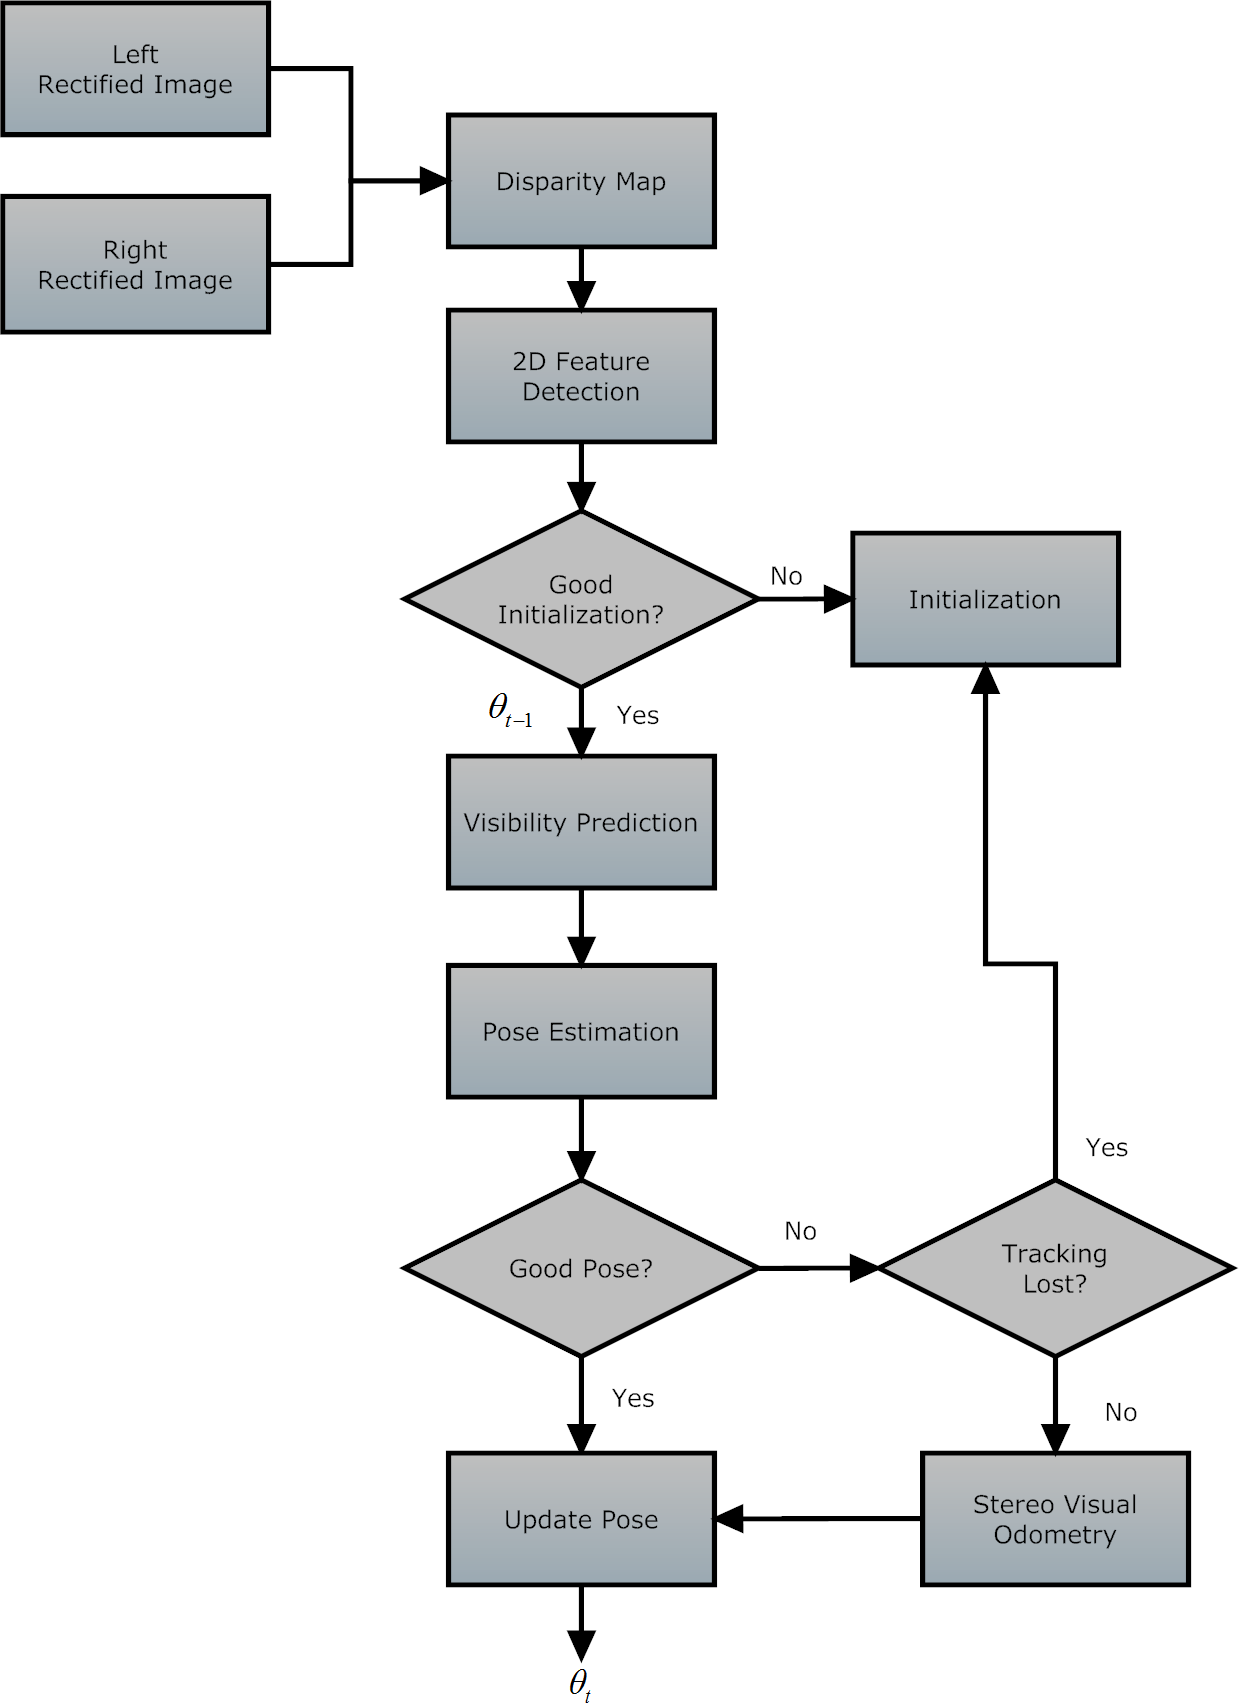
\includegraphics[width=\linewidth]{images/vision_based_localization.png}
%  \end{center}
%  \caption{Overall overview of our vision-based localization framework with visibility prediction.\label{fig:vision_localization}}
%\end{figure}
%
